\chapter{Mechanical Advantage, Gears, and Hydraulics}

\section{Mechanical Advantage}

\index{mechanical advantage}Mechanical advantage is the ratio between the force output 
by the machine and the force the user puts into the machine:
$$ MA = \frac{F_{out}}{F_{in}} = \frac{Load}{Effort}$$

Since the input force is \textit{applied} to the simple machine, sometimes the 
input force is called an applied force and abbreviated as $F_a$. For example, 
you only need to apply a relatively little force to your car's brakes in order 
for the hydraulic braking system to apply enough force to your tires to stop 
them spinning (we'll examine this further below). 

\subsection{What does it mean to work hard?}
Humans use simple machines to ``make work easier", but what does this mean in a 
physics sense? Does using a machine actually decrease the amount of work the 
user has to do? When we say a task is easier, we usually mean \textit{we have to 
apply less force}. You might say that it is ``less work" to push something up a 
shallow incline than up a steep incline. But does the person pushing \textit{
actually do less work} (in a physics sense), or does that work simply require 
a smaller force? We'll answer this question by examining the physics of incline 
planes below, and the results will be true for all simple machines. 

Ideally we want a higher Mechanical Advantage, which means we are putting in less input force for a greater output force.
\section{Gears}
Gears are rotating parts of machines that transmit torque or other types of rotational motion through intertwined teeth. \index{gears}Often gears are meshed together; two or more meshed gears are referred to as a gear train.\index{gear train}

Gears have teeth that mesh with each other. When you apply torque to one gear, 
it transfers torque to the other. The resulting torque is increased or decreased 
depending on the ratio of the number of teeth on the gears. We will go in depth on torque in a future chapter, but know that torque depends on the radius of the gear, and the radius of a gear is proportional to the number of teeth, the tooth count directly controls the torque.

\subsection{Involute Gears}
Gear teeth have a very unique shape. The vast majority of modern gears use what is known as an \textbf{\newterm{involute gear profile}}.\index{involute gear} An involute gear is one whose tooth shape is derived from the \emph{involute of a circle}. This curve is generated by imagining a fixed string being unwrapped from the circumference of a circle. The path traced by the end of the string forms the involute.

\begin{figure}[H]
    \centering
    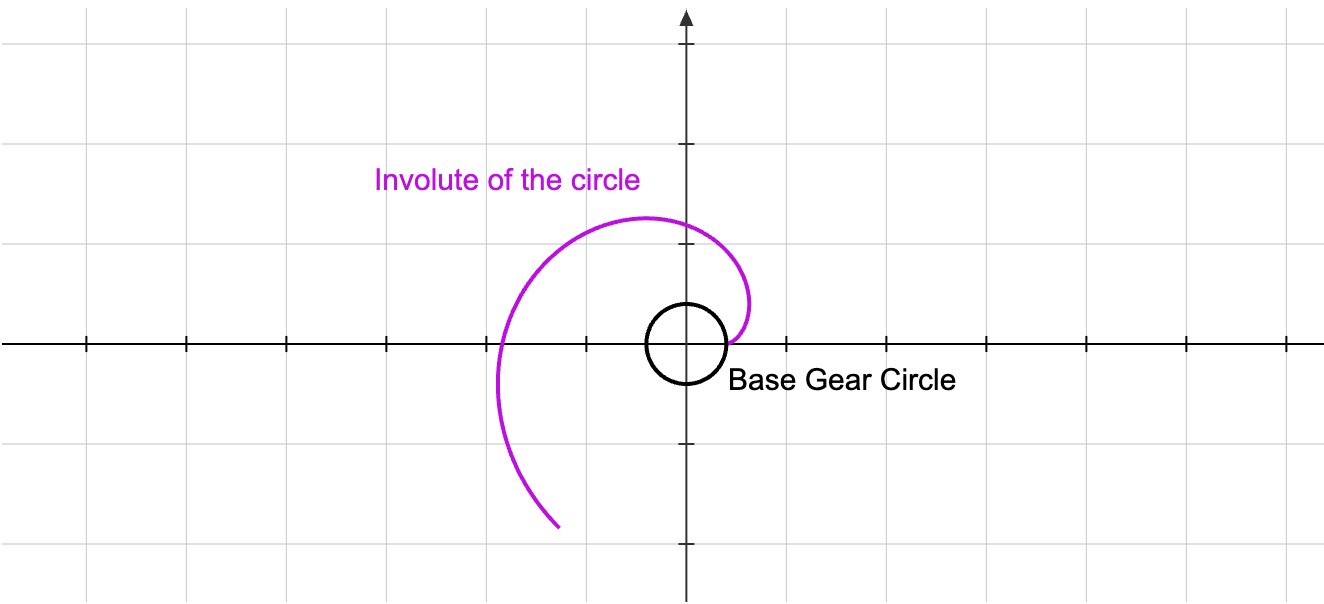
\includegraphics[width=0.8\textwidth]{involute.png}
    \caption{The involute of a circle shown. The purple line is revolved for $4\pi$ radians or $2$ revolutions (for clarity).}
    \label{fig:involute}
\end{figure}

Although the involute curve resembles a spiral, it is not an Archimedean spiral. Instead, its geometry is defined by the constant unwrapping of the string, which gives the involute several important mechanical properties.

The primary advantage of the involute profile shape is that it ensures smooth and reliable torque transfer between two or more meshing gears. When two involute gears engage, their teeth make contact at a single point that moves along a straight line known as the \textbf{line of action}. This line is tangent to the base circles of both gears. As the gears rotate, the point of contact travels along this line while maintaining a constant pressure angle, which allows the gears to transmit motion at a constant speed ratio even if the center distance between them varies slightly. 

Some more gear construction terminology:
\begin{description}
    \item[The pressure angle] The acute angle between the line of action and a normal to the line connecting the gear centers. May vary depending on the involute shape, but most commonly $20^\circ$. 
    \item[Addendum] The difference between the pitch circle and its tooth tip circle.
    \item[Dedendum] The difference between the radius of the pitch circle of a gear and its root circle
    \item[Tooth Height] The distance between its root circle and the tip are called the tooth height (h).
    \item[Total Height of Tooth] The total height of the gear is the sum of the addendum (ha = 1.00m) and the dedendum (hf = 1.25m).
\end{description}

FIXME Possible gear diagram in tikz with labeled everything

\begin{figure}[H]
    \centering
    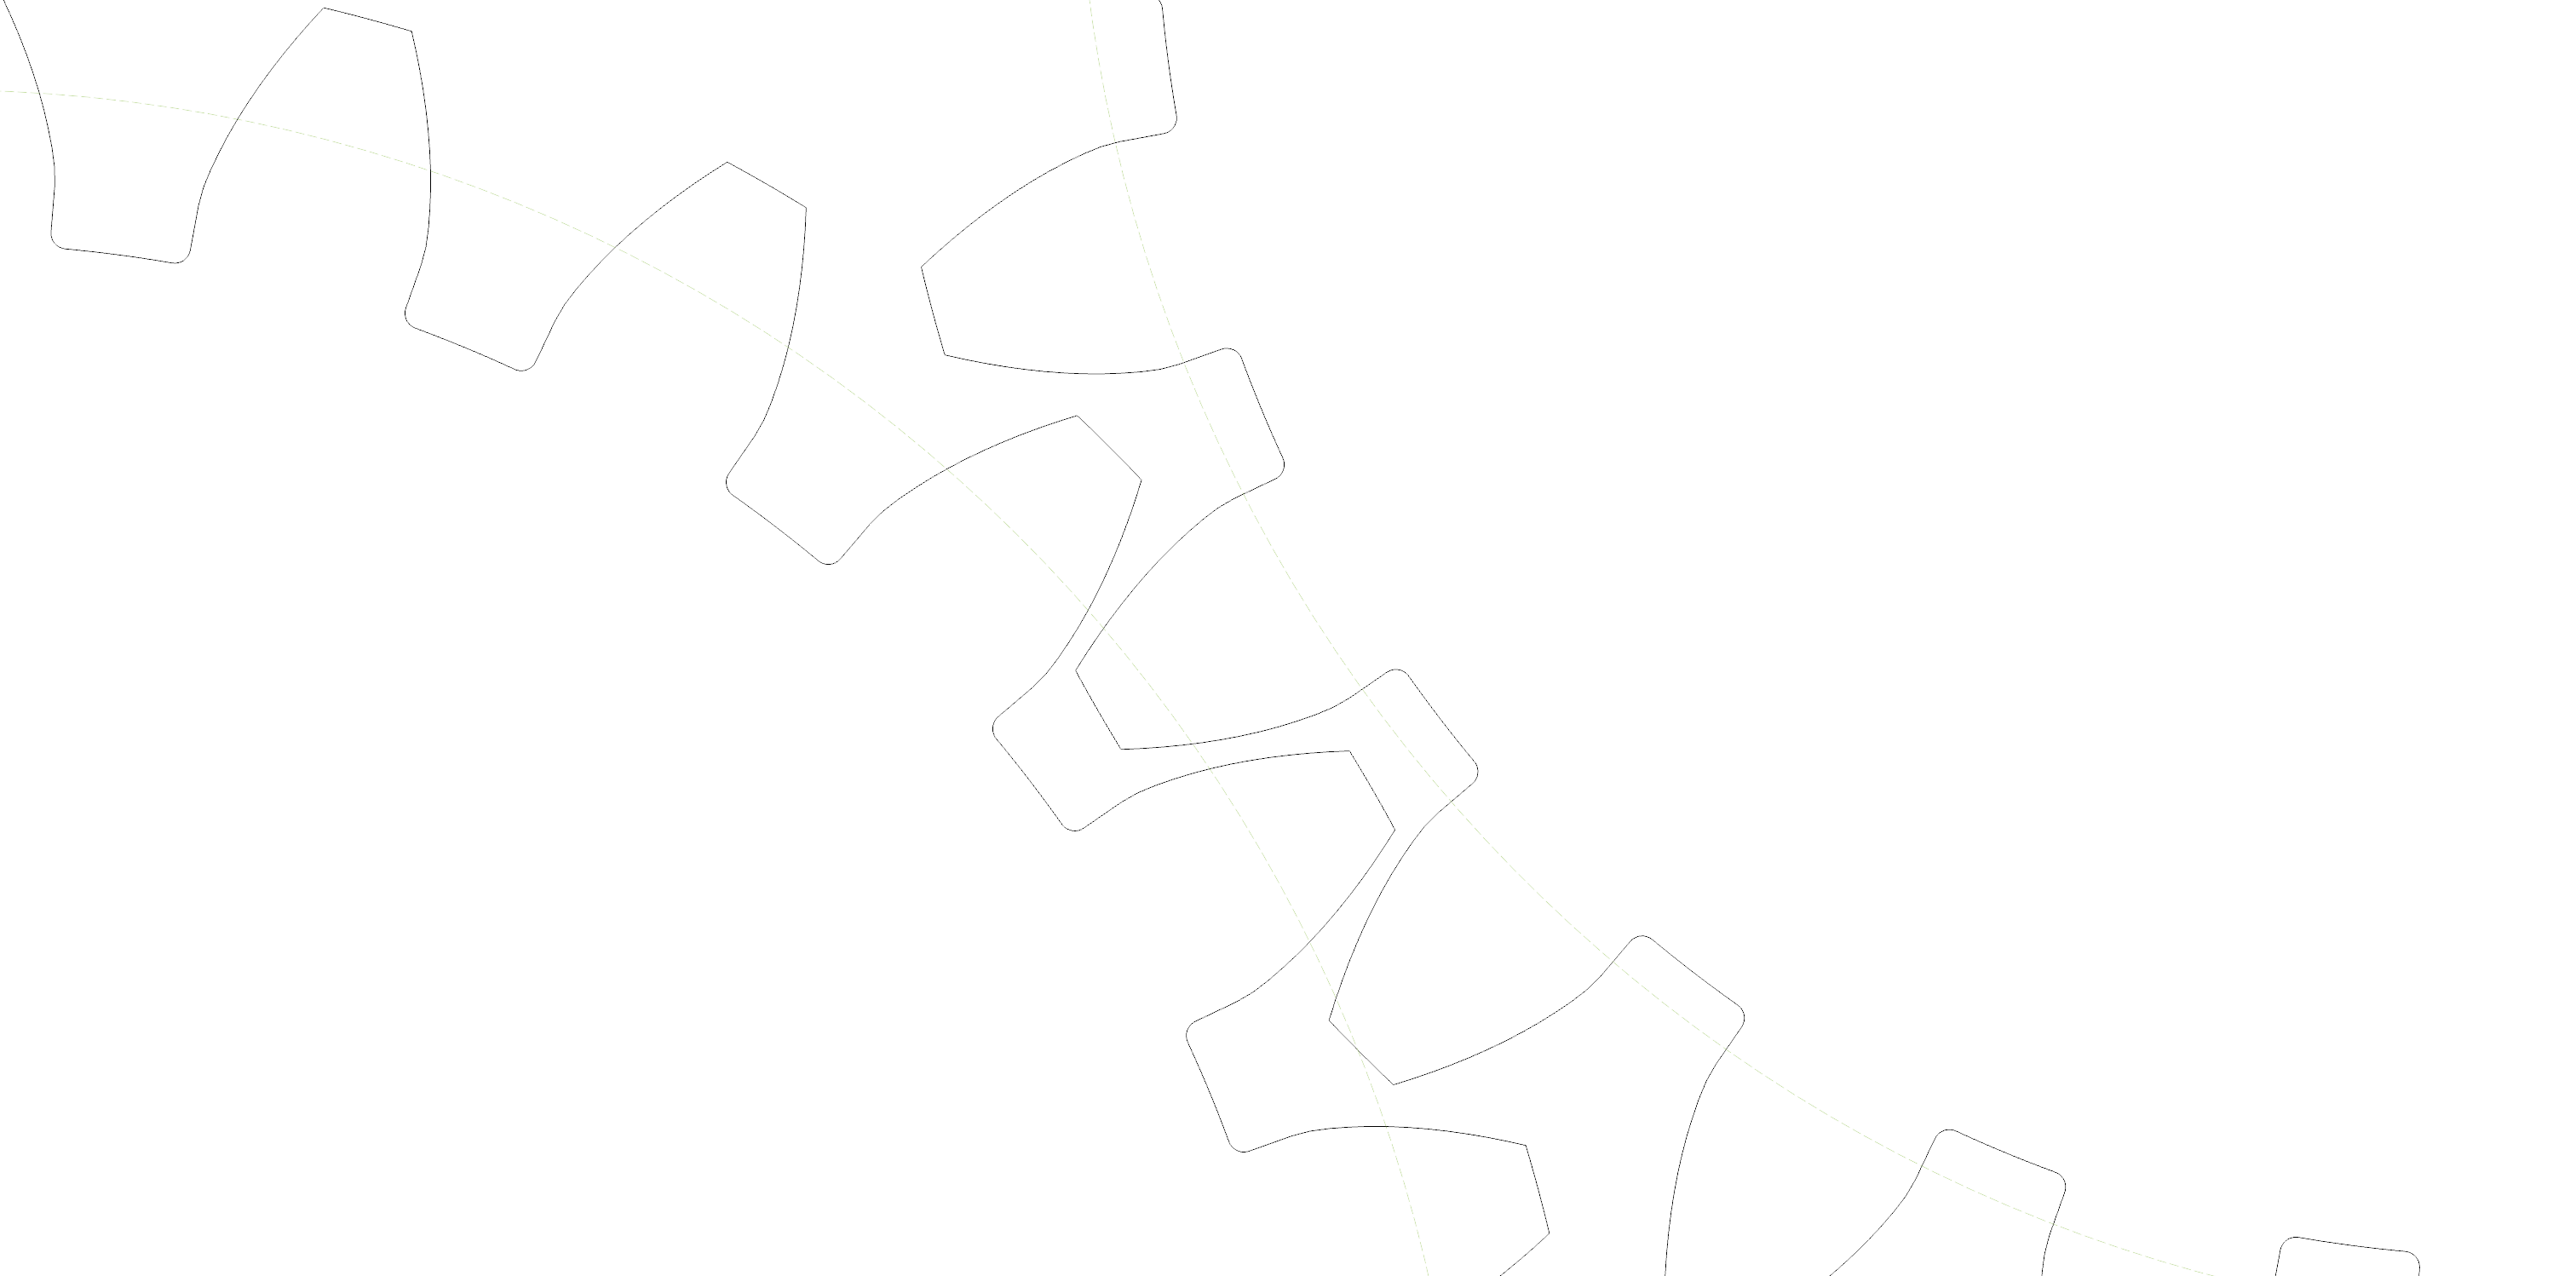
\includegraphics[width=0.9\textwidth]{Gears.png}
    \caption{Two gears meshing together diagram (not directly conjoined for clarity).}
    \label{fig:gears2}
\end{figure}
For part of the motion, Gear One pushes Gear Two down. Once the contact point passes the midpoint of the line of action, Gear One pushes up on Gear Two. This causes a constant transfer of torque.

FIXME Diagram of this

%this may be daunting but I included it for reference
A parametric function, defined by $x(\theta)$ and $y(\theta)$ is given by 
\[
\begin{bmatrix}
    x(\theta) \\
    y(\theta)
\end{bmatrix}
= r \begin{bmatrix}
    \cos(\theta) \\
    \sin(\theta)
\end{bmatrix}
+ r \theta  \begin{bmatrix}
    \sin(\theta) \\
    -cos(\theta)
\end{bmatrix}
\]

For gears, a large torque makes it easier to start rotating an object or to continue rotating it against resistance, such as climbing a hill or accelerating a heavy load.

\textbf{Power}, on the other hand, measures how quickly work is being done. In rotational motion, power depends on both torque and rotational speed. A system can produce high torque at low speed, or lower torque at high speed, and still deliver the same power.

Gears allow a machine to adjust this balance between torque and speed without significantly changing the power being transmitted (neglecting losses). When gears increase torque, they reduce rotational speed, and visa versa.

A familiar example is riding a bicycle up a hill. When climbing, it becomes difficult to pedal in a high gear because the torque required at the pedals is large. Shifting to a lower gear increases the torque applied to the rear wheel for the same pedaling effort, making it easier to climb. However, the pedals must turn more times for each rotation of the wheel, so the bicycle moves more slowly. The rider's power output remains roughly the same, but it is delivered as higher torque at lower speed.

The same principle applies to the gears in a car. When starting from rest or climbing a steep incline, a low gear is used to provide high torque at the wheels, allowing the vehicle to overcome inertia and gravity. At highway speeds, higher gears are used to reduce torque and increase speed, improving efficiency and reducing engine wear. In both cases, the engine produces power, and the transmission adjusts how that power is distributed between torque and rotational speed.

In mechanical systems, gears therefore do not create power; instead, they shape how power is delivered.

\begin{figure}[H]
    \centering
    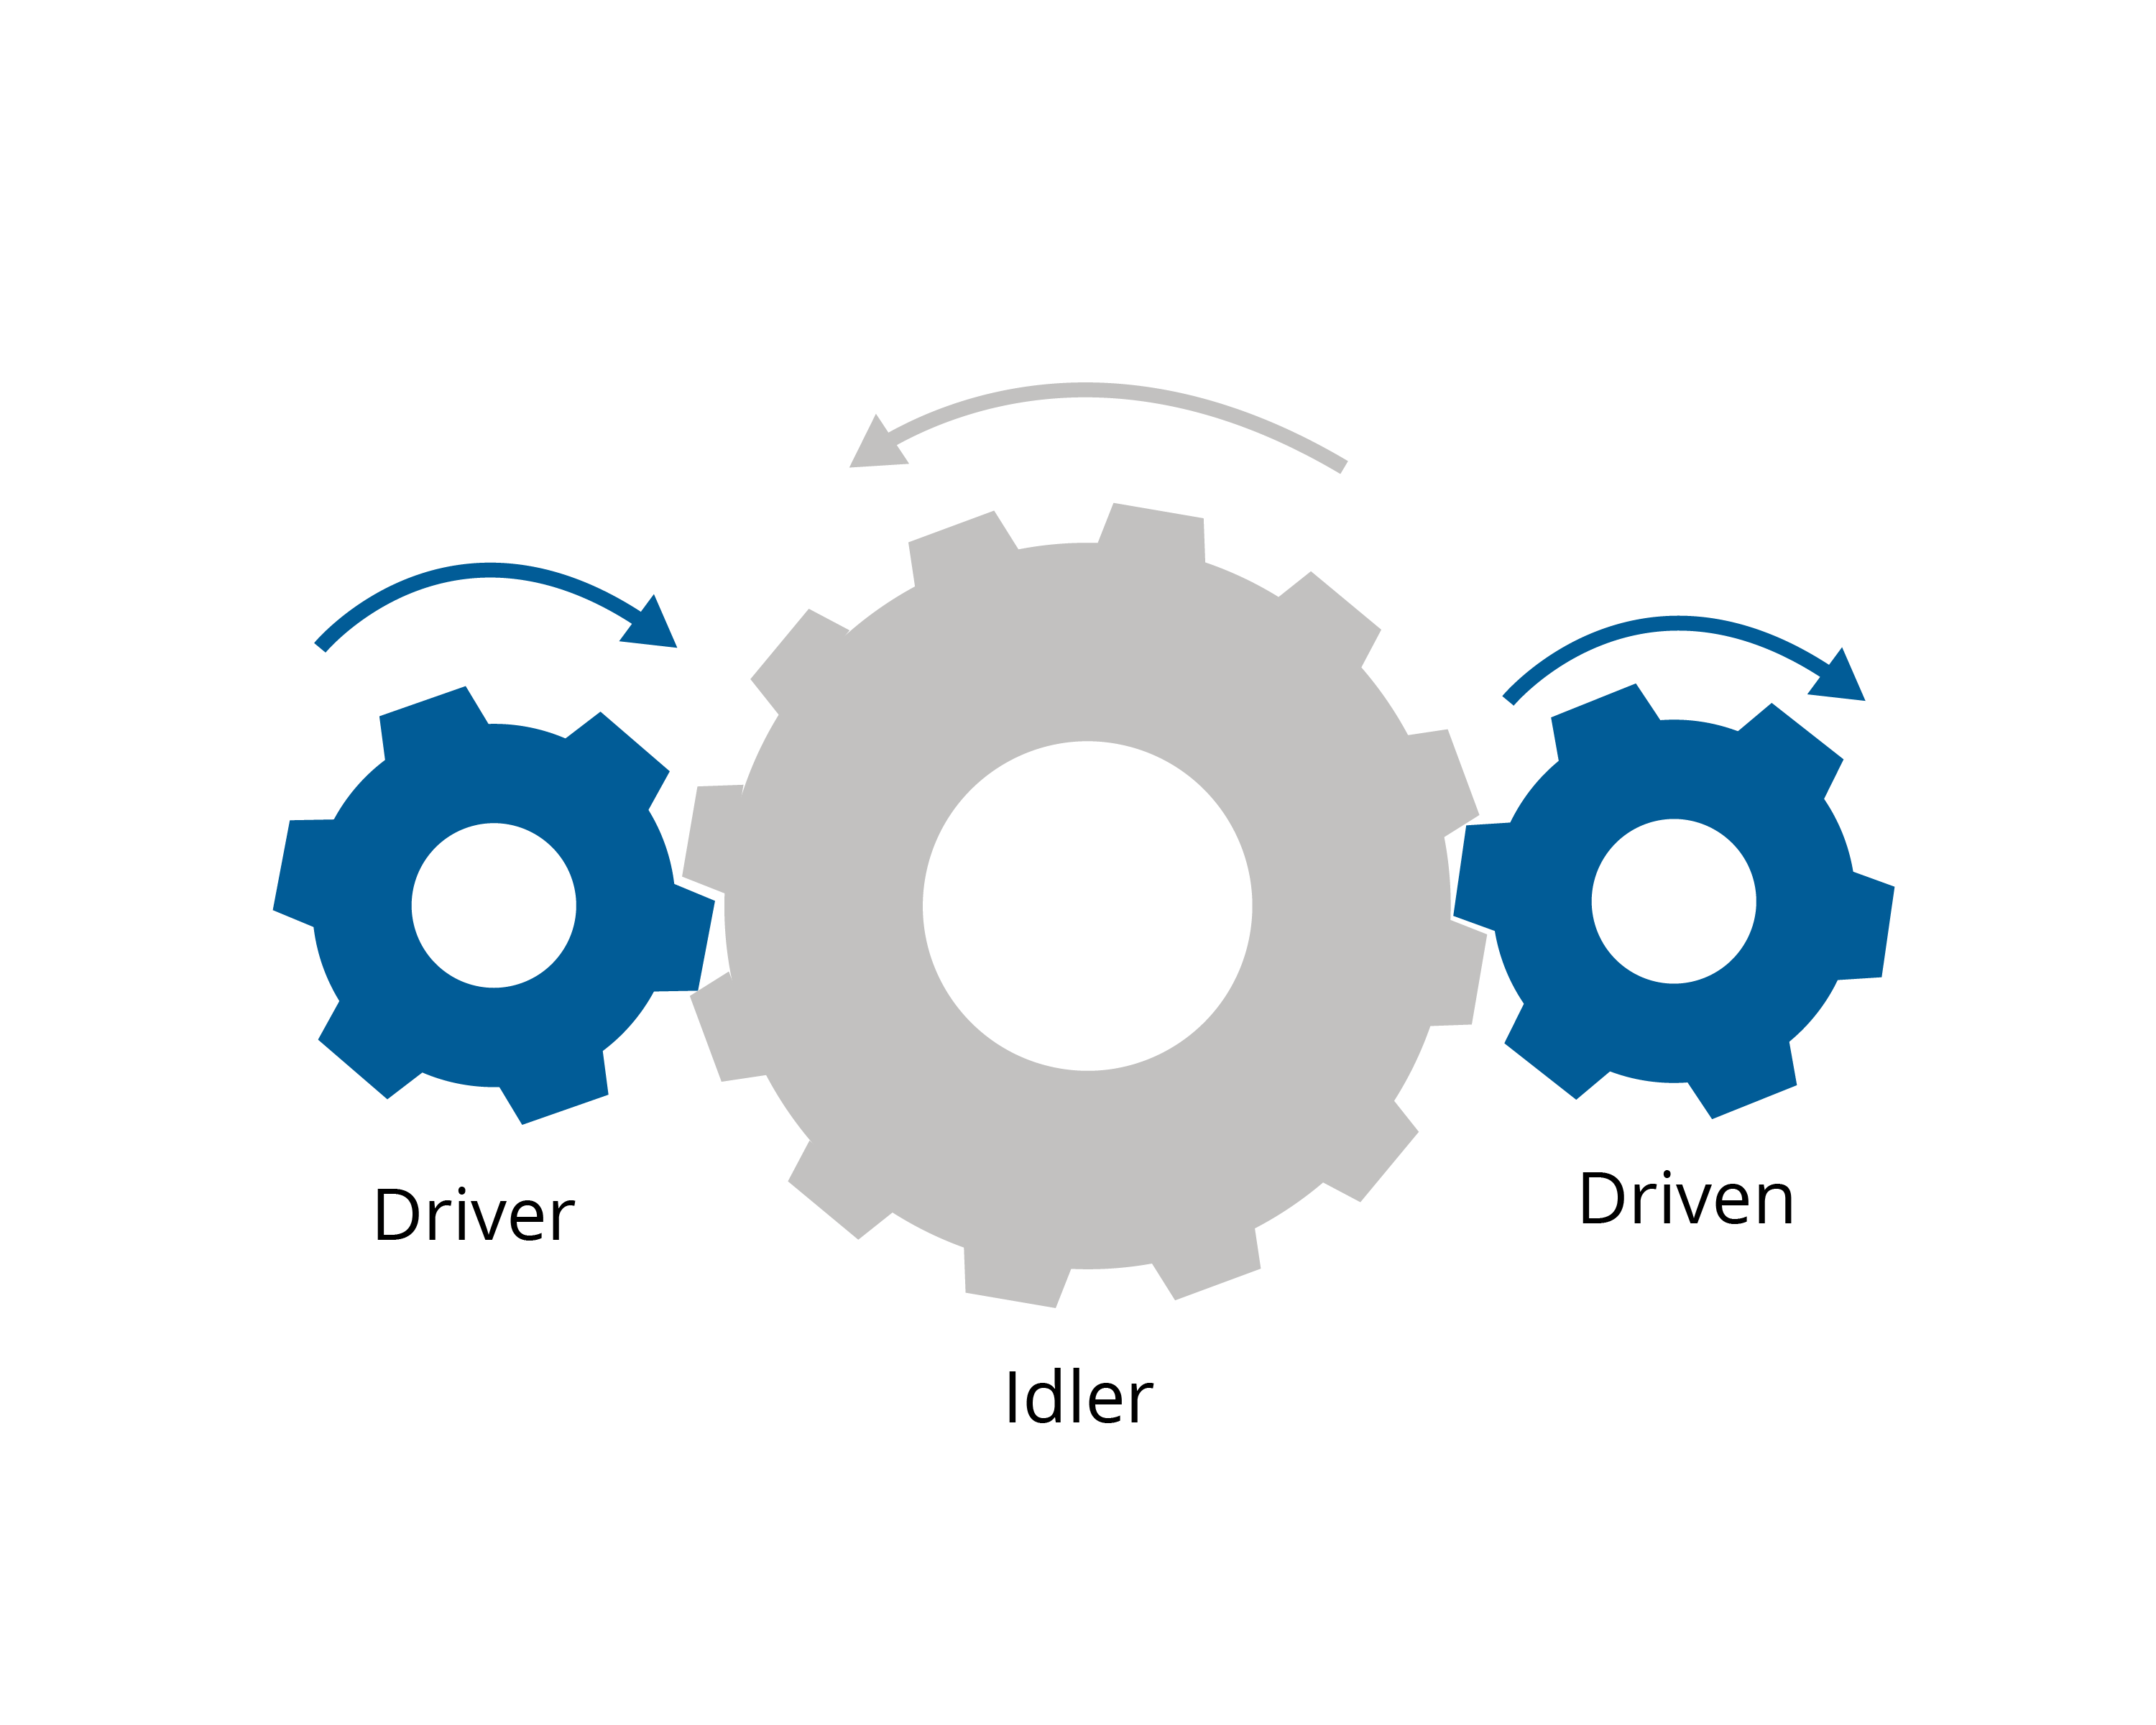
\includegraphics[width=0.7\textwidth]{gearsNew.png}
    \caption{.}
    \label{fig:gears}
\end{figure}
\subsection{Teeth}
If \( N_A \) is the number of teeth on the gear you are turning with a torque of 
\( T_A \), and \( N_L \) is the number of teeth on the gear it is turning, the resulting torque is:

\[
T_L = \frac{N_A}{N_L} T_A
\]
% maybe add more on this? not sure how important it is or if it needs to be emphasized more
\begin{Exercise}[title={Gears}, label=gear]
In a bicycle, the goal is not always to gain mechanical advantage, but to spin 
the pedals slower while applying more force.

You like to pedal your bike at 70 revolutions per minute. The chainring 
connected to your pedals has 53 teeth. The circumference of your tire is 2.2 
meters. You want to ride at 583 meters per minute.

How many teeth should the rear sprocket have?
\end{Exercise}
\begin{Answer}[ref=gear]
The equation relating these quantities is:

\[
583 = 70 \times 2.2 \times \frac{53}{n}
\]

Solving for \( n \), we find \( n = 14 \) teeth.
\end{Answer}

% Content about rack and pinion? Maybe...

\section{Hydraulics}

In a \index{hydraulic system}hydraulic system, such as a car's braking system, you exert force on a 
piston filled with fluid. The fluid transmits this pressure into another 
cylinder, where it pushes yet another piston that moves the load. The pressure 
at each end of the hydraulic system must be the same. 
\begin{figure}[H]
    \centering
    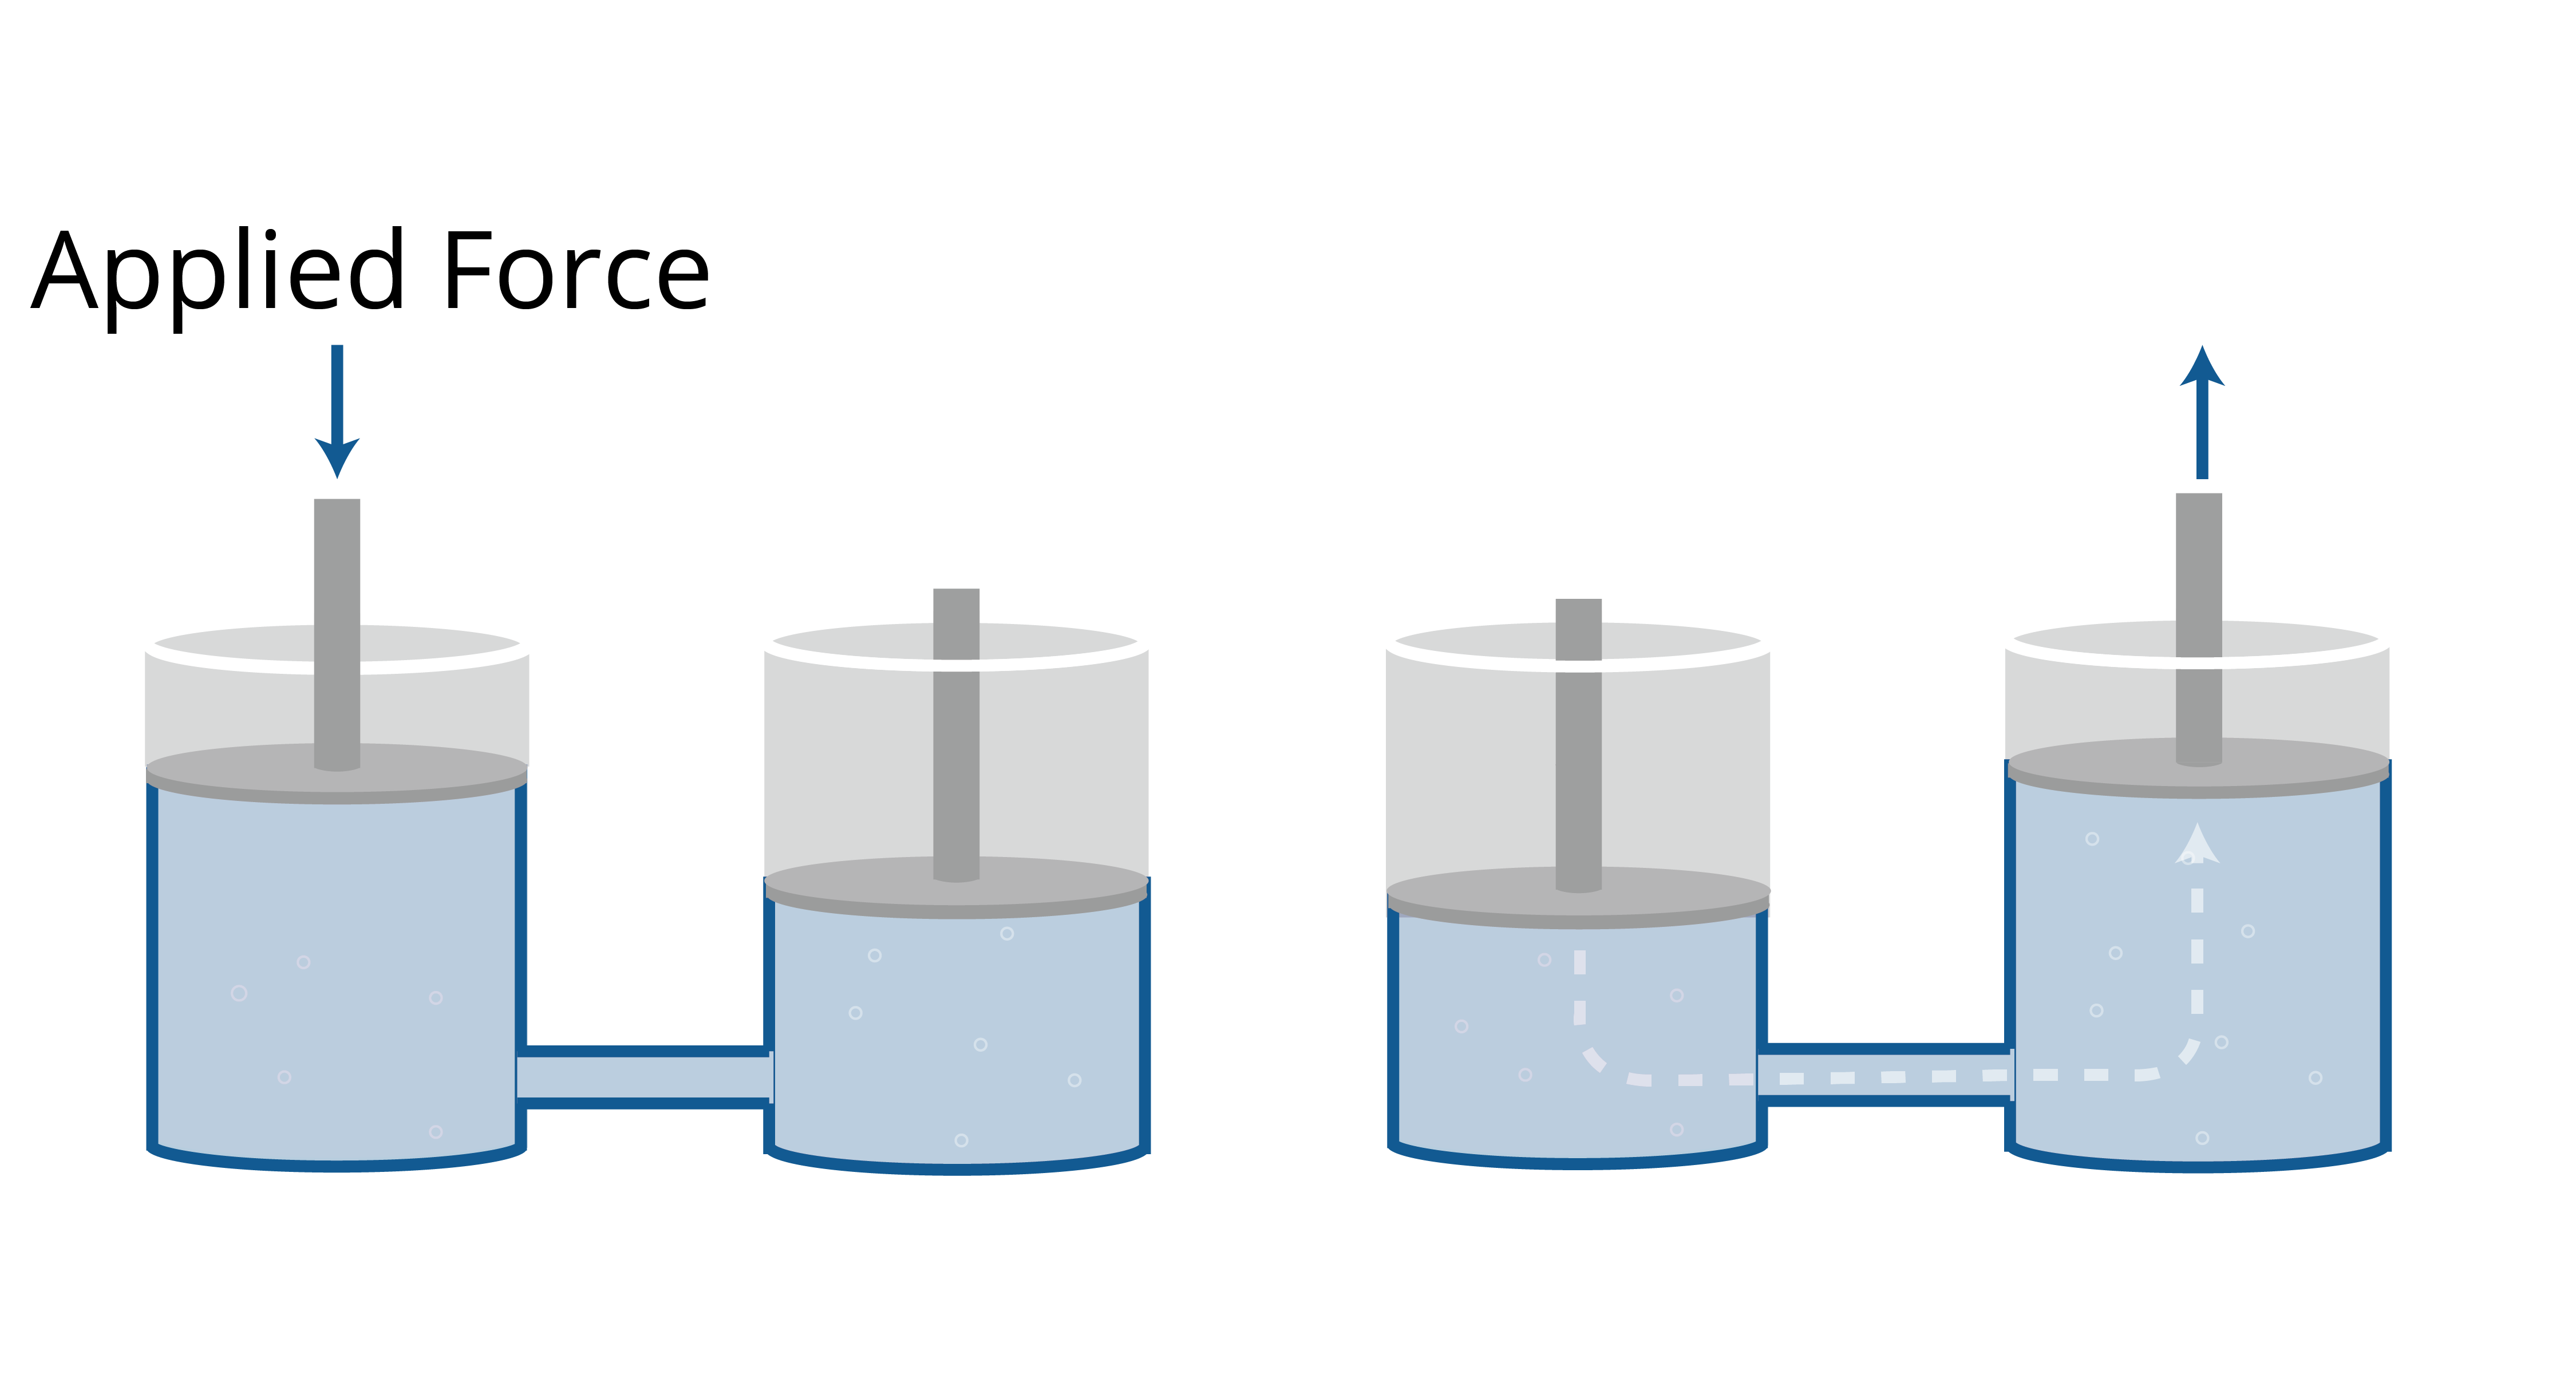
\includegraphics[width=\textwidth]{hydraulicsNew.png}
    \caption{A diagram showing the transfer of fluid from one container to the other.}
    \label{fig:hydraulics}
\end{figure}

\newterm{Pressure} is force applied to an area; it is calculated by dividing 
the force by the area.  The pressure in the fluid is typically measured in 
pascals (Pa), which is equivalent to \(N / m^2\). We will use pascals for this 
calculation.

To calculate the pressure you create, divide the force applied $F_{a}$ by the 
area of the piston head $A$. To determine the force on the other piston, 
multiply the pressure by the area of the second piston.
% added equation for pressure

\begin{equation}
    P = \frac{F_{a_1}}{A_1} = \frac{F_{a_2}}{A_2}
\end{equation}


\begin{Exercise}[title={Hydraulics}, label=hydraulics]
Your car has disc brakes. When you apply 2,500,000 pascals of pressure to the 
brake fluid, the car stops quickly. As the car designer, you want this to 
require only 12 newtons of force from the driver's foot.

What should the radius of the master cylinder (the piston the driver pushes) be?
\end{Exercise}
\begin{Answer}[ref=hydraulics]
We are solving for the radius \( r \) of the piston. The area of the piston is 
\( \pi r^2 \), so the pressure is:

\[
\text{Pressure} = \frac{12}{\pi r^2}
\]

Setting the pressure equal to 2,500,000 pascals:

\[
2,500,000 = \frac{12}{\pi r^2}
\]

Solving for \( r \), we find:

\[
r = \sqrt{\frac{12}{\pi \times 2.5 \times 10^6}} \approx 0.00124 \text{ meters}.
\]
\end{Answer}
